
\chapter{Desenvolvimento e Resultados}

Este capítulo descreve o desenvolvimento do projeto proposto. O projeto é composto por 5 tarefas de implementação:

\begin{itemize}
    \item Montar os \textit{datasets} de \textit{barcodes} e números;
    \item Treinar, avaliar e selecionar o melhor modelo de rede neural para \textit{barcodes} e números;
    \item Implementar o algoritmo de detecção dos \textit{barcodes}.
    \item Implementar o algoritmo de detecção dos números.
    \item Implementar a aplicação web
\end{itemize}

Utilizaremos a Figura \ref{fig:imagemBase} como referência para a explicação do sistema ao longo do capítulo.

\begin{figure}[h!]
	\centering
	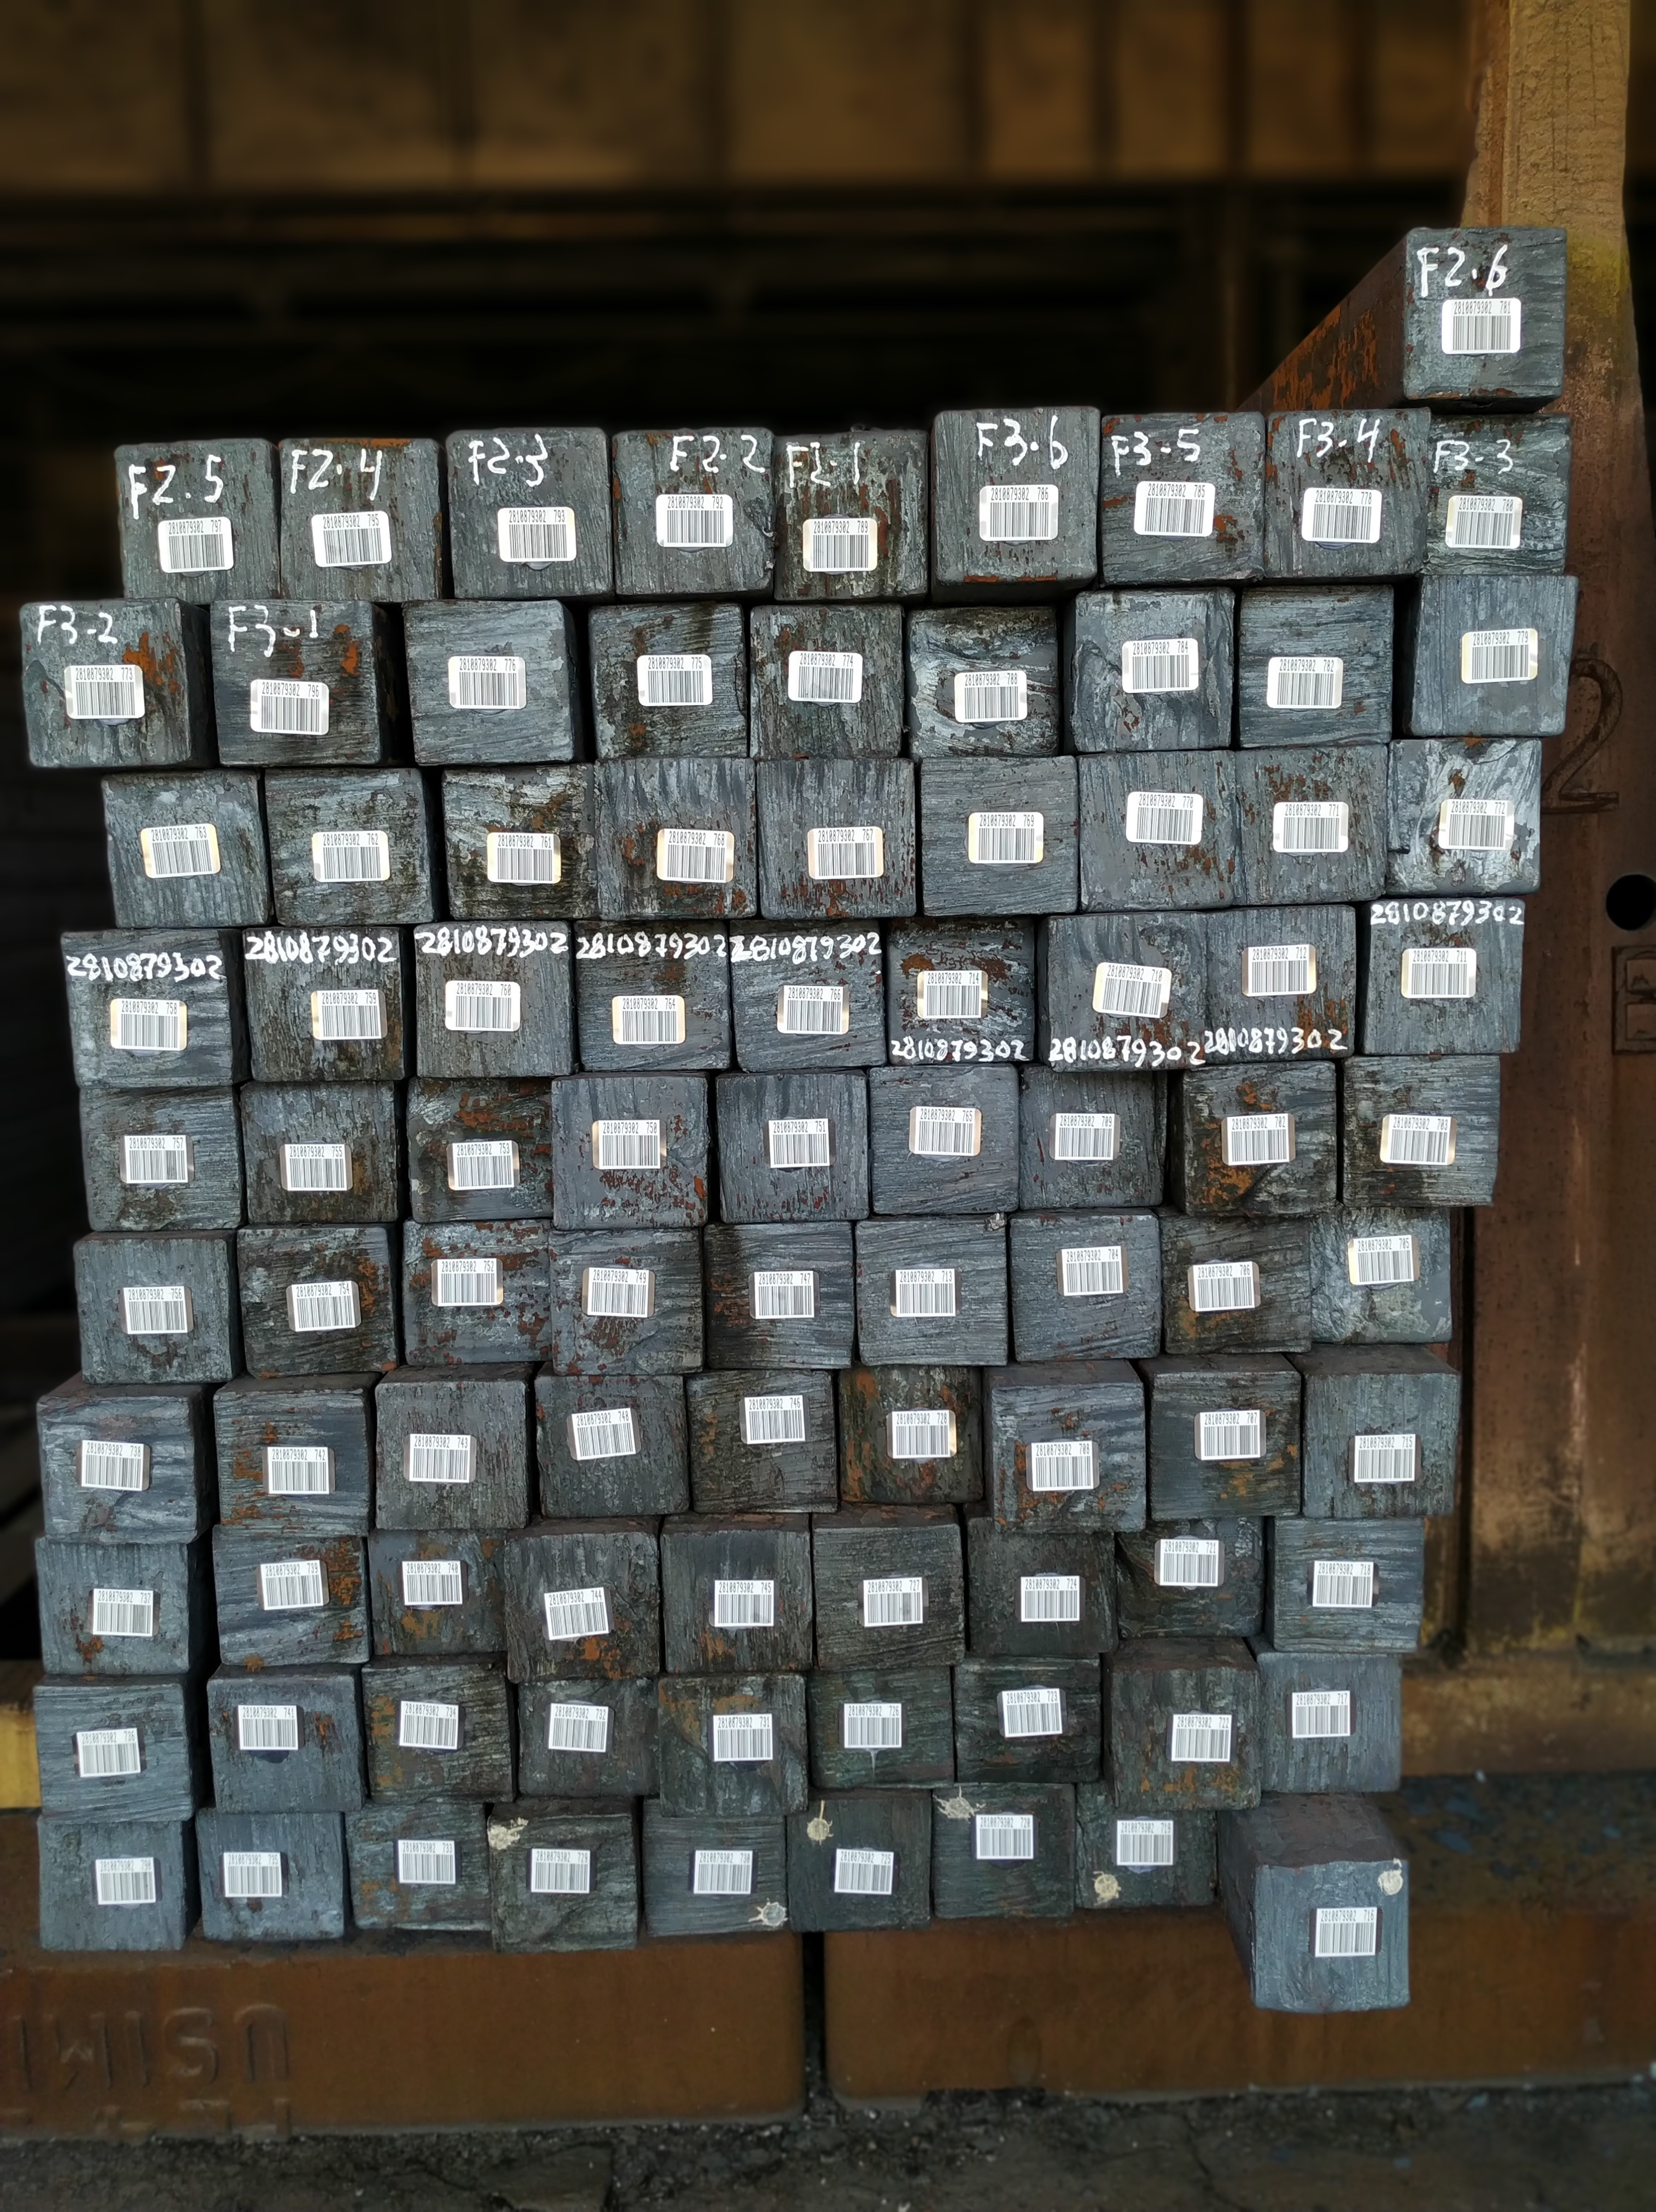
\includegraphics[width=0.5\linewidth]{figuras/img1.jpg}
	\caption{Foto tirada da corrida de tarugos.}
	\label{fig:imagemBase}
\end{figure}

\section{Montagem dos \textit{datasets}}

Nesta seção faremos a montagem dos dois \textit{datasets} para que, posteriormente, as redes neurais sejam treinadas. 

Inicialmente faremos o \textit{download} do conjunto de dados de \textit{barcodes} disponibilizado pelo laboratório \citeauthor{Arte-Lab}. Teremos por volta de 500 imagens de código de barras para o nosso \textit{dataset} inicial.

Criaremos pastas no seguinte modelo de divisão para nosso \textit{dataset}. (Código \ref{cod:folders})
\begin{lstlisting}[caption=Divisão dos arquivos para dataset, label=cod:folders][htb!]
        +---barcode
        |   +---train
        |   |   +---annotations
        |   |   \---images
        |   \---validation
        |       +---annotations
        |       \---images
        
        +---number
        |   +---train
        |   |   +---annotations
        |   |   \---images
        |   \---validation
        |       +---annotations
        |       \---images
\end{lstlisting}

Através do método \textit{Data Augmentation} \ref{sec:dataAugm}, aumentaremos nossa base de dados para que, após o treino, a acurácia do modelo de nossa rede neural seja a maior possível. Aplicaremos o modelo nas imagens 500 imagens resultando em $\sim~1500$ imagens de código de barras.

Utilizando a Figura \ref{fig:imagemBase}, cortaremos as etiquetas com a ajuda do software \textit{Paint} do \textit{Windows}, para sera gerada nossa base de dados de números. Optamos por utilizar os números localizados nas etiquetas uma vez que foram feitos diversos treinamento com fontes numéricas diferentes e, portanto, não obtivemos uma acurácia de detecção do número esperada.(Figura \ref{fig:barcodeDataset})

\begin{figure}[htbp]
	\centering
	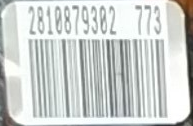
\includegraphics[width=0.25\linewidth]{figuras/MachineLearning/barcodeDataset.png}
	\caption{Montagem \textit{dataset} de números}
	\label{fig:barcodeDataset}
\end{figure}

Colocaremos 75\% das imagens na pasta validation e resto em train tanto no \textit{dataset} de \textit{barcodes} como no de números.

\subsection{Anotações das imagens}

Utilizando o software LabelImg (Subseção \ref{sub:LabelImg}), faremos as anotações das imagens para que seja gerado o arquivo PASCAL VOC no formato XML. (Figura \ref{fig:barNumAn})

\begin{figure}[htbp]
	\centering
	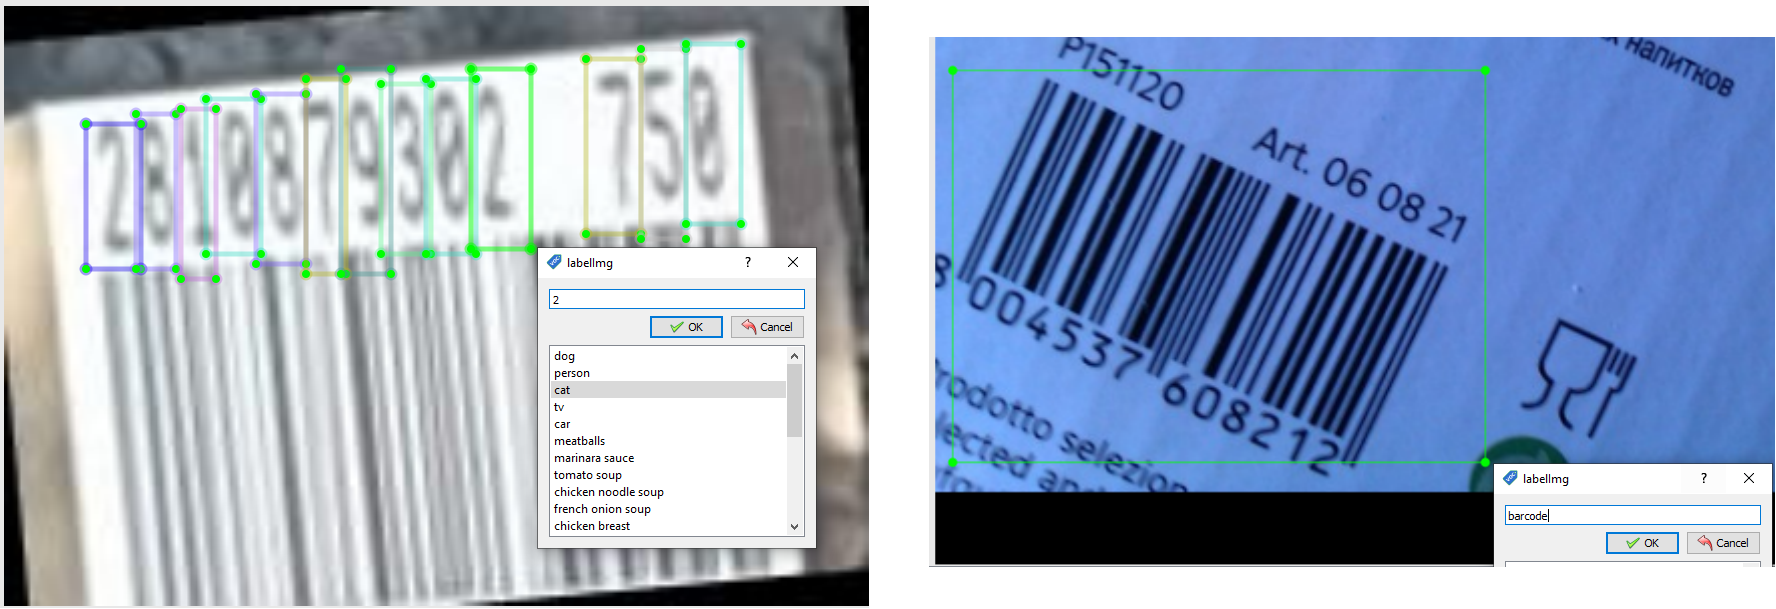
\includegraphics[width=1\linewidth]{figuras/MachineLearning/barNumAn.png}
	\caption{Anotações das imagens (Números e \textit{Barcodes})}
	\label{fig:barNumAn}
\end{figure}

\section{Fase de treinamento}

Nesta seção iremos treinar, avaliar e selecionar o melhor modelo de \textit{barcode} e número a partir da rede neural pré-treinada YOLOv3 (Subseção \ref{sub:Yolov3}).

\subsection{Treinando o modelo}

Utilizando a biblioteca ImageAI, e importando a classe \textit{DetectionModelTrainer}, treinaremos o modelo (Código \ref{cod:modeTrain}).

\begin{lstlisting}[caption=Exemplo de código do método \textit{data augmentation}, label=cod:modeTrain][htb!]
from imageai.Detection.Custom import DetectionModelTrainer

trainer = DetectionModelTrainer()
trainer.setModelTypeAsYOLOv3()
trainer.setDataDirectory(data_directory="barcode")
trainer.setTrainConfig(object_names_array=["barcode"], batch_size=4, 
                        num_experiments=11, 
                        train_from_pretrained_model=
                                            "pretrained-yolov3.h5")
trainer.trainModel()
\end{lstlisting}

\begin{itemize}
    \item \textit{object\_names\_array}: matriz que contém os nomes dos objetos em nosso \textit{dataset};
    \item \textit{batch\_size}: indica o tamanho do \textit{batch} para o treinamento;
    \item \textit{num\_experiments}: indica o número de vezes que a rede treinará sobre todas as imagens de treinamento, também chamadas de \textit{Epochs};
\end{itemize}

\begin{figure}[htbp]
	\centering
	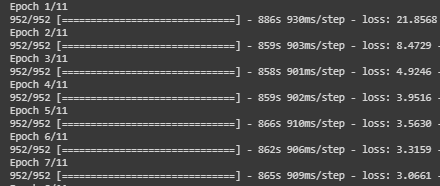
\includegraphics[width=1\linewidth]{figuras/MachineLearning/barcodeTraining.png}
	\caption{Anotações das imagens (Números e \textit{Barcodes})}
	\label{fig:barTrain}
\end{figure}

    A figura acima significa o progresso do treinamento.
\begin{itemize}
    \item Para cada experimento (\textit{Epoch}), a perda total geral de validação (por exemplo - \textit{loss}: 4.7582) é relatada.
    \item Para cada queda em \textit{loss} após uma experiência, um modelo é salvo na pasta barcode/models. Quanto menor a perda, melhor o modelo, de um modo geral, é desenhada para mostrar o quão longe estamos da solução "ideal". 
\end{itemize}

O método \textit{trainer.evaluateModel} mostrará as métricas de saída de cada modelo e a partir dos modelos gerados, avaliaremos o mAP \footnote{AP (precisão média) é uma métrica popular na medição da precisão de detectores de objetos;} de cada modelo de detecção salvo.  (Código \ref{cod:metrics})

\begin{lstlisting}[caption=Métricas de saída do modelo, label=cod:metrics][htb!]
metrics = trainer.evaluateModel(model_path="detection_model-ex-013--loss-0003.066.h5", json_path="detection_config_barcode.json", iou_threshold=0.5, object_threshold=0.3, nms_threshold=0.5)
\end{lstlisting}

Obtivemos o seguintes resultados para nossos modelos de barcodes e números:

\begin{table}[H]
	\centering
	\begin{tabular}{|l|l|l|}
		\hline
		\rowcolor[HTML]{ECF4FF} 
		\multicolumn{1}{|c|}{\cellcolor[HTML]{ECF4FF}\textit{Característica}} &
		\multicolumn{1}{|c|}{\cellcolor[HTML]{ECF4FF}\textit{Barcode}} & \multicolumn{1}{c|}{\cellcolor[HTML]{ECF4FF}\textit{Number}}\\ \hline
		\textit{Epochs} & 7 & 53\\ \hline
		\textit{Loss} & 3.066 & 12.296\\ \hline
		\textit{mAP} & 91.07\% & 77.90\%  \\ \hline
	\end{tabular}
	\caption{Melhores resultados encontrados nos modelos.}
	\label{tab:Result}
\end{table}

Ao detalhar a média de precisão dos números, podemos observar a porcentagem da probabilidade de cada número.

\begin{table}[H]
	\centering
	\begin{tabular}{|l|l|l|}
		\hline
		\rowcolor[HTML]{ECF4FF} 
		\multicolumn{1}{|c|}{\cellcolor[HTML]{ECF4FF}\textit{\textit{Number}}} &
		\multicolumn{1}{|c|}{\cellcolor[HTML]{ECF4FF}\textit{Média}}\\ \hline 
		0&  78.38\% \\ \hline
		1&  49.64\% \\ \hline
		2&  85.21\% \\ \hline
		3&  78.55\%\\ \hline
		4&  83.47\% \\ \hline
		5&  67.46\% \\ \hline
		6&  80.00\% \\ \hline
		7&  85.66\% \\ \hline
		8&  84.31\% \\ \hline
		9&  86.36\% \\ \hline
		mAP&  77.90\% \\ \hline 
		
	\end{tabular}
	\caption{Médias de precisões dos números.}
	\label{tab:avgNumbersResult}
\end{table}


\section{Implementação dos algoritmos de detecção}

Nesta seção iremos implementar os algoritmos de detecção de \textit{barcodes} e números utilizando os modelos de redes reunais treinadas na seção anterior. Para que o sistema complete o fluxo e entregue os dados à aplicação WEB de forma correta, será necessário \textit{scripts} \footnote{Programas escritos para um sistema de tempo de execução especial que automatiza a execução de tarefas que poderiam alternativamente ser executadas uma por vez por um operador humano.} de criações de pastas ao longo das etapas.

O cógido é disponibilizado através do link: \textbf{\textit{shorturl.at/bluOV}}

\subsection*{Divisão dos arquivos}

A arquitetura de pastas do sistema de detecção foi pensada e desenvolvida de acordo com as necessidades que o sistema web teria para que pudesse ter uma boa comunicação entre os serviços. (Figura \ref{fig:folderSystem})

\begin{figure}[H]
	\centering
	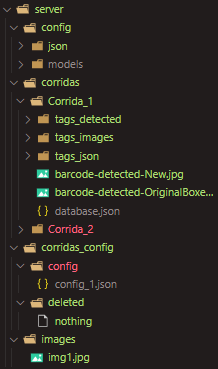
\includegraphics[width=0.4\linewidth]{figuras/MachineLearning/folderSystem.png}
	\caption{Divisão dos arquivos do sistema de detecção}
	\label{fig:folderSystem}
\end{figure}


\begin{itemize}
    \item \textbf{config}: Arquivos de configuração do sistema como os modelos de \textit{barcode} e números e os arquivos JSON de configuração para treinar a rede.
    \item \textbf{corridas}: Pastas contendo todas as corridas corridas.
    \begin{itemize}
        \item \textbf{Corrida\_1}
            \begin{itemize}
                \item \textbf{tags\_detected}: Imagens das etiquetas recortadas contendo as \textit{bounding boxes} dos números;
                \item \textbf{tags\_images}: Imagens das etiquetas recortadas;
                \item \textbf{tags\_json}: Arquivos  de configuração de cada etiqueta como, por exemplo, números detectados, accurácias, posições das \textit{bounding boxes} de cada número.
                \item \textbf{barcode-detected-New.jpg}: Imagem contendo as \textit{bounding boxes} aumentadas pelo script.
                \item \textbf{barcode-detected-OriginalBoxes.jpg}: Imagem contendo as \textit{bounding boxes} originais.
                \item \textbf{database.json}: Arquivo resumindo as configurações das etiquetas que se encontram na pasta "/tags\_json".
            \end{itemize}
    \end{itemize}
     \item \textbf{corridas\_config}
        \begin{itemize}
            \item \textbf{config}: Arquivos de configuração resumo de cada corrida para consumo o sistema web;
            \item \textbf{deleted}: Pasta referente as corridas que forem deletadas pelo sistema web;
        \end{itemize}
    \item \textbf{images}: Pasta contendo todas as imagens que são \textit{input} do sistema. (Ex: Figura \ref{fig:imagemBase})
\end{itemize}



\subsection{Detecção de \textit{barcode}}

Inicialmente para que seja detectado os códigos de barras, será criada funções para verificar se a mesma \textit{bounding box} está sendo detectada duas ou mais vezes. Para isso, faremos uma função de interseção sobre união entre duas \textit{bounding boxes}, comparando cada uma com todas as outras existentes na imagem. Assim, caso seja retornado um valor diferente de zero da função, uma \textit{bounding box} será deletada. (Código \ref{ap:IoU})

Ao iniciar o treinamento do modelo, identificamos que as \textit{bounding boxes} estavam ficando menores que a etiqueta (Figura \ref{fig:bboxNew}) e tivemos que aumentar 50 \textit{pixels} em cada uma manualmente para que seja recortada a etiquetada com os números que serão detectados posteriormente. (Código \ref{ap:AumentaBbox})

\begin{figure}[H]
	\centering
	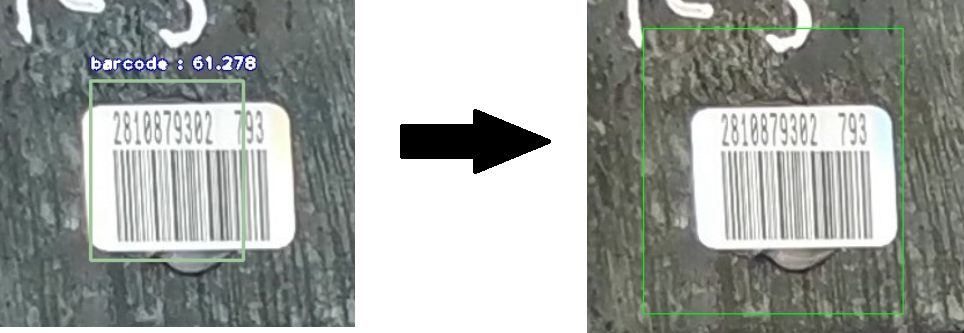
\includegraphics[width=1\linewidth]{figuras/MachineLearning/bboxNew.png}
	\caption{ Resultado do aumento das \textit{bounding boxes}}
	\label{fig:bboxNew}
\end{figure}

Cada imagem de \textit{bounding boxes} serão salvas na pasta "/tags\_images" para que seja utilizada pelo modelo de detecção de números na próxima etapa.

O resultado da saída do modelo da rede neural de \textit{barcodes} é o nome do objeto detectado, a acurácia e a posição da bounding box de cada código de barras. (Figura \ref{fig:indentBarcodes})

\begin{figure}[H]
	\centering
	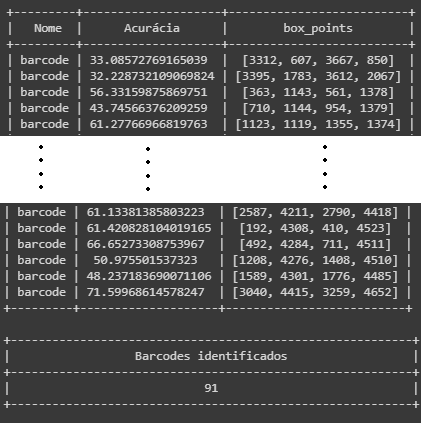
\includegraphics[width=0.6\linewidth]{figuras/MachineLearning/indentBarcodes.png}
	\caption{ Resultado do modelo de detecção de barcodes}
	\label{fig:indentBarcodes}
\end{figure}


\subsection{Detecção de número}


O algoritmo de detecção de números utilizará as imagens que foram recortadas pelo modelo anterior que estão localizados na pasta "/tags\_images". 

Semelhante ao modelo de detecção de \textit{barcodes}, verificamos que pela posição das \textit{bounding boxes} dos números nas etiquetas, podemos afirmar que cada número estava sendo identificado mais de uma vez. (Figura \ref{fig:numDup})

\begin{figure}[H]
	\centering
	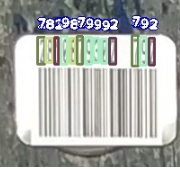
\includegraphics[width=0.4\linewidth]{figuras/MachineLearning/numDup.png}
	\caption{Etiqueta com múltiplas detecções de números}
	\label{fig:numDup}
\end{figure}

Para solucionar este problema, desenvolvemos uma função que calcula a coordenada central de cada \textit{bounding box} dos números e aplicamos a equação de Distância Euclidiana \footnote{Distância entre dois pontos.} para saber a distância entre duas \textit{bounding boxes}. 

\begin{equation} 
dist(x_{i}, x_{j}) = \sqrt{(x_{i1} - x_{j1})^2 + (x_{i2} - x_{j2})^2 +...+ (x_{ir} - x_{jr})^2}.
\label{eq: euclid}
\end{equation}

Ao identificar que dois números foram detectados duas vezes, iremos escolher o número com maior acurácia para que possamos ter certeza que aquele número é provavelmente o número correto. (Código \ref{ap:removeNumber})

No final da execução do \textit{script} de remoção de números duplicados, verificamos a quantidade de números identificados na etiqueta, pois ainda pode ser que haja algum número duplicado que não conseguimos identificar devido estar fora do parâmetro de comparação estabelecido por nós como distância entre dois números. 

Como em cada etiqueta temos 13 números, o \textit{script} verifica se a quantidade total de números detectados pelo modelo é igual a 13, pois enquanto não for, serão deletados os número com menor acurácia até que o total de números seja 13. (Código \ref{ap:identNumber})

Também é gravada uma \textit{flag} \footnote{Mecanismo lógico que funciona como semáforo: uma entidade (objeto) detém como ativa uma determinada \textit{flag} se a característica associada a essa \textit{flag} estiver presente.} de alerta em cada número da etiqueta caso a acurácia seja menor que 98\% para que seja mostrada pelo \textit{front-end} para que o usuario fique alerta a essa etiqueta pois pode ser que esteja errada.

\begin{figure}[H]
	\centering
	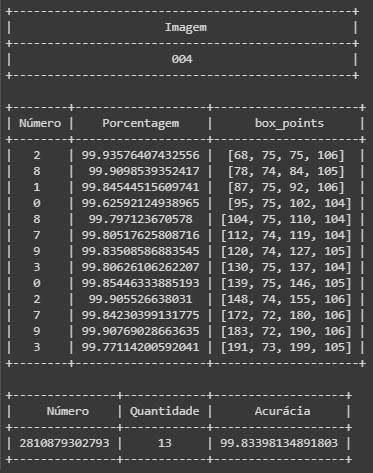
\includegraphics[width=0.53\linewidth]{figuras/MachineLearning/imageTag.png}
	\caption{\textit{Output} de uma das imagens do algoritmo de detecção de números.}
	\label{fig:imageTag}
\end{figure}

O resultado da saída do modelo da rede neural de números que é gravado em um arquivo "database.json", são objetos detectados (números), a acurácia, a posição da \textit{bounding box} e a \textit{flag} de alerta de cada número. (Figura \ref{fig:imageTag})

\section{Aplicação Web}

O propósito desta aplicação é para que o usuário final tenha o controle detalhado de forma automática facilitando a conferência das corridas que foram já foram coletadas.

Nesta seção são apresentadas as etapas de desenvolvimento dos microsserviços utilizados no sistema elaborado, assim como o \textit{back-end} e o \textit{front-end}. 

\subsection*{Divisão dos arquivos}

Os microsserviços desenvolvidos foram projetados para seguir a \textit{Clean Architecture}. Esta arquitetura consiste em dividir as responsabilidades dentro de uma aplicação, encapsulando e abstraindo o código para facilitar a leitura e entendimento das devidas funções de cada arquivo \cite{martin2000clean}.

\begin{figure}[htbp]
	\centering
	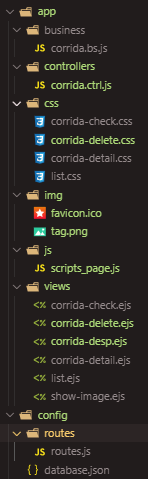
\includegraphics[width=0.22\linewidth]{figuras/WebService/cleanArchtecture.png}
	\caption{Divisão dos arquivos do Sistema Web}
	\label{fig:cleanArchtecture}
\end{figure}

É possível ver a divisão dos arquivos utilizando a \textit{Clean Architecture} do Sistema Web na Figura \ref{fig:cleanArchtecture}. Explicando esta divisão, na pasta config/routes encontram-se as configuração das rotas que são utilizadas no sistema, nos \textit{controllers}, são feitas o tratamento dos \textit{inputs} e respostas das rotas, redirecionando para os \textit{business}, que é onde está a lógica principal da aplicação. No arquivo database.json é onde acontece a interação com o banco de dados. 

O \textit{front-end} da aplicação se encontra nas pastas css, js e views, sendo responsáveis pela interface gráfica do sistema.

\subsection{Back-end}

Nesta seção iremos tratar da regra de negócio do sistema, bem como a comunicação com banco de dados que estão gravados em arquivos JSON\footnote{Javascript Object Notation (JSON), é um formato compacto de troca de dados simples e rápida entre sistema}.

As operações são realizadas através dos \textit{endpoints}, que é uma forma de comunicação entre os sistemas. O sistema os disponibiliza como endereços para acesso, que podem receber e enviar informações, dependendo do que foi programado. (Tabela \ref{tab:endpoints})

Utilizaremos a \textit{engine} EJS para que o \textit{back-end}, em Node.JS, comunique com \textit{front-end} através do consumos\footnote{O termo "consumir um \textit{endpoint}" significa enviar informações para o \textit{endpoint}, esperando algum retorno, de sucesso ou falha.} dos \textit{endpoints}.

\begin{table}[H]
	\centering
	\begin{tabular}{|l|l|}
		\hline
		\rowcolor[HTML]{ECF4FF} 
		\multicolumn{1}{|c|}{\cellcolor[HTML]{ECF4FF}\textit{Endpoint}} & \multicolumn{1}{c|}{\cellcolor[HTML]{ECF4FF}Característica} \\ \hline
		/ & \begin{tabular}[c]{@{}l@{}} retorna a lista de corridas existentes e redireciona\\ para \textit{home-page}\end{tabular}\\ \hline
		/corrida-detail & \begin{tabular}[c]{@{}l@{}}retorna os detalhes da corrida selecionada e redireciona\\ para tela \textit{corrida-detail}\end{tabular} \\ \hline
		/corrida-check & \begin{tabular}[c]{@{}l@{}} despacha a corrida e salva no banco de dados o\\ status "Despachada"\end{tabular} \\ \hline
		/corrida-delete & \begin{tabular}[c]{@{}l@{}} deleta a corrida e move seu arquivo "config\_x.json"\\ para pasta /deleted\\\end{tabular}\\ \hline
		/show-image & \begin{tabular}[c]{@{}l@{}}redireciona para tela de edição da etiqueta\end{tabular}\\ \hline
		/edit-image & possibilita a edição do número da etiqueta\\ \hline
		/upload-image & \begin{tabular}[c]{@{}l@{}}carrega uma foto para dar \textit{start} no sistema de \\reconhecimento de objetos. \\\end{tabular}\\ \hline
	\end{tabular}
	\caption{\textit{Endpoints} do sistema WEB.}
	\label{tab:endpoints}
\end{table}

Os \textit{controllers} possuem módulos que são responsáveis pela renderização, navegação das paginas através dos \textit{endpoints}, bem como no envio de dados para o navegador.

Os \textit{business} são os responsáveis pelas regras de negócio do sistema de modo que cada método tenha uma função especifica. Comunicação entre os aquivos JSON e listagem dos objetos são suas principais funções.

\subsection{Front-end}

Nesta seção será apresentada as telas e suas funcionalidades utilizando o \textit{frontend} da aplicação. No desenvolvimento foi utilizada as tecnologias HTML, CSS, JavaScript e EJS, responsável pela comunicação entre \textit{frontend} e \textit{backend}.

A tela inicial do sistema é composta pela lista de corridas que já foram identificadas e pelo componente responsável por fazer o \textit{upload}\footnote{ação de enviar um arquivo para determinado local.} de uma nova imagem.(Figura \ref{fig:list1})

A imagem será enviada para a pasta \textit{images} (Figura \ref{fig:folderSystem}) e automaticamente treinada pelo sistema de detecção.

Toda corrida que é inicialmente treinada, terá o status como "Inadimplente", pois ainda não foi despachada para as Laminações. Dessa forma, o sistema terá diversas opções para que o usuário tenha total controle da mesma.

A lista de corridas tem como funcionalidade as opções de visualizar detalhadamente ou deletar a corrida escolhida. Caso a corrida seja deletada, a tela será redirecionada para tela de \textit{delete}(Figura \ref{fig:corrida_delete}) e no \textit{backend} o arquivo config\_x.json é movido para pasta \textit{deleted}(Figura \ref{fig:folderSystem}).

\begin{figure}[H]
	\centering
	\includegraphics[width=1\linewidth]{figuras/WebService/Screens/list  1.png}
	\caption{Componente para \textit{upload} de novas imagens}
	\label{fig:list1}
\end{figure}

\begin{figure}[H]
	\centering
	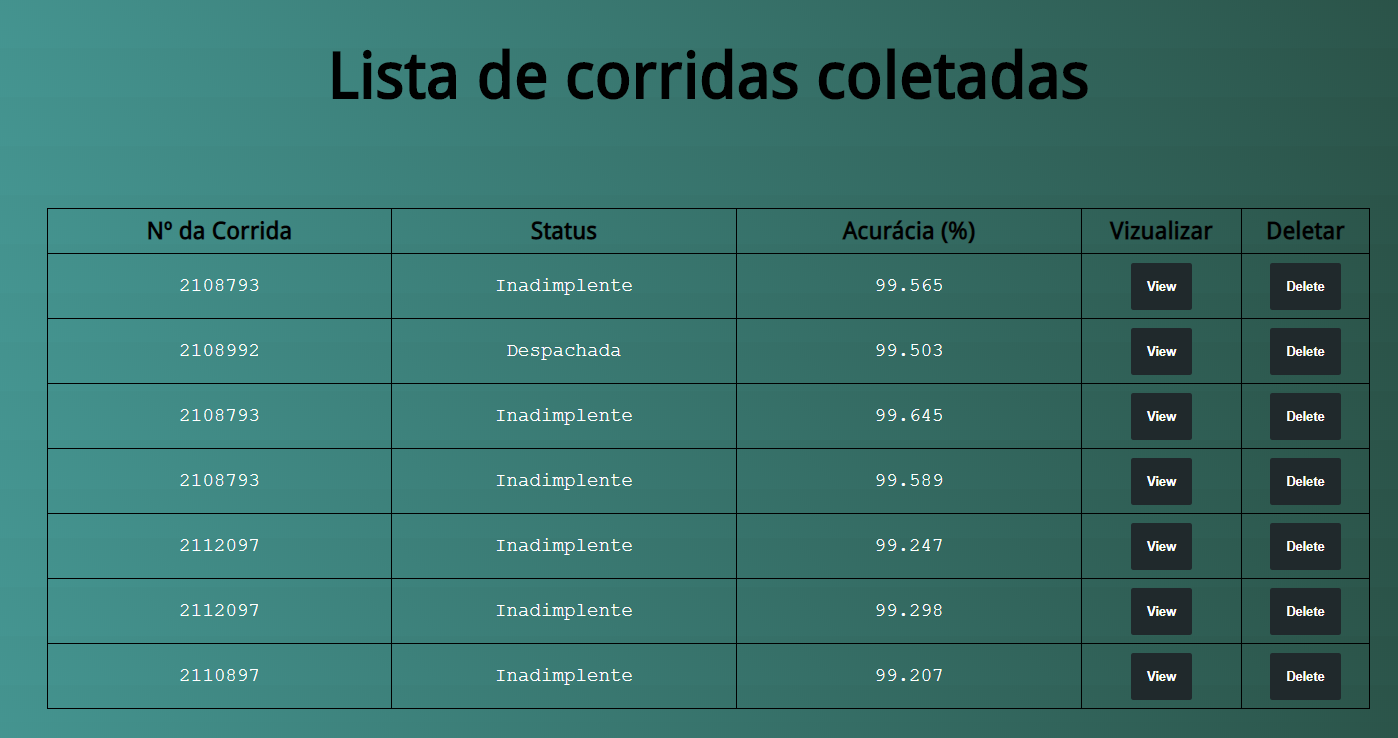
\includegraphics[width=1\linewidth]{figuras/WebService/Screens/list 2.png}
	\caption{Lista de corridas coletadas}
	\label{fig:list2}
\end{figure}

\begin{figure}[H]
	\centering
	
\includegraphics[width=0.5\linewidth]{figuras/WebService/Screens/corrida_delete.png}
	\caption{Corrida deletada.}
	\label{fig:corrida_delete}
\end{figure}

A segunda tela é o detalhamento da corrida em que é mostrado o número da corrida, a quantidade de peças, a acurácia média das etiquetas e o status atual. (Figura \ref{fig:detalCorrida})

\begin{figure}[H]
	\centering
	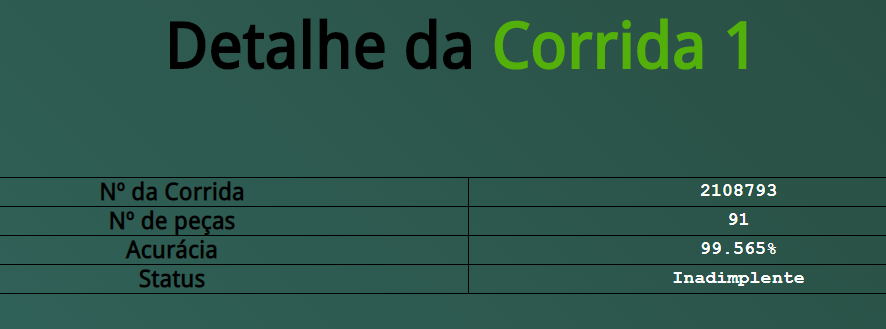
\includegraphics[width=0.8\linewidth]{figuras/WebService/Screens/detail 1.png}
	\caption{Detalhamento da corrida selecionada}
	\label{fig:detalCorrida}
\end{figure}

Na mesma tela de detalhamento, é mostrada todas as peças (etiquetas) que foram detectadas pelo sistema de detecção. A lista detalha o identificador, o número da peça que é referente ao número localizado acima do código de barras da etiqueta, a acurácia de cada uma e um botão para visualizar a imagem da etiqueta.(Figura \ref{fig:detail2.1})

Cada etiqueta tem como característica, caso algum algarismo tenha acurácia menor que 98\%, o fundo da cédula preenchido pela cor vermelha, alertando o usuário que possivelmente aquela etiqueta tem um número que foi detectado erroneamente.

O botão despachar tem a função de despachar a corrida e alterar seu status para "Despachada" no banco de dados (Figura \ref{fig:corrida_desp}). Caso o status da corrida já esteja como "Despachada", o sistema redirecionará o usuário para tela de erro com a seguinte mensagem (Figura \ref{fig:corrida_desp_x}) 

\begin{figure}[H]
	\centering
	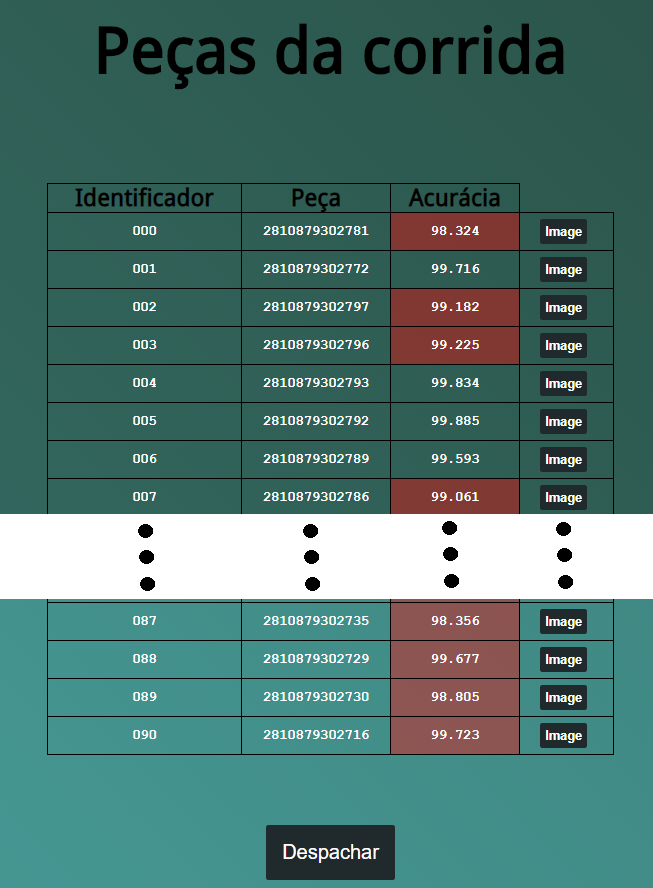
\includegraphics[width=0.65\linewidth]{figuras/WebService/Screens/detail 2.1.png}
	\caption{Detalhamento das peças da corrida}
	\label{fig:detail2.1}
\end{figure}

\begin{figure}[H]
	\centering
	
\includegraphics[width=0.5\linewidth]{figuras/WebService/Screens/corrida_desp.png}
	\caption{Corrida despachada pelo usuário}
	\label{fig:corrida_desp}
\end{figure}

\begin{figure}[H]
	\centering
	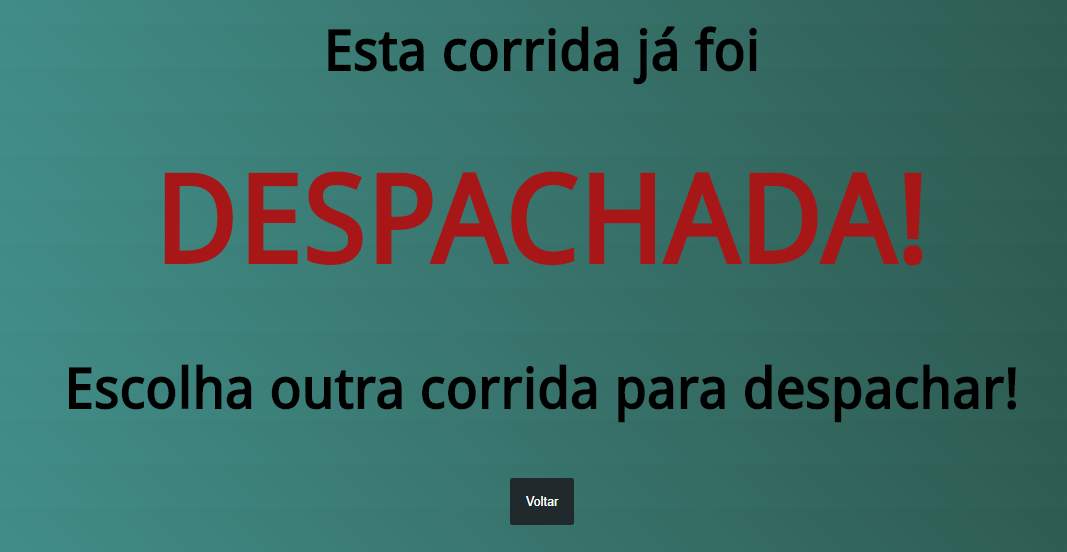
\includegraphics[width=0.5\linewidth]{figuras/WebService/Screens/corrida_desp_X.png}
	\caption{Mensagem de erro para status de corrida despachada}
	\label{fig:corrida_desp_x}
\end{figure}

A última tela do sistema é referente ao detalhamento da etiqueta que foi escolhida através do botão "\textit{Image}".

Nesta tela, o usuário terá permissão para editar a etiqueta caso tenha identificado que há algum algarismo numérico detectado que seja diferente da imagem ao lado.

Ao salvar ele será redirecionado para tela de detalhamento da corrida para que então continue o procedimento de, verificar as outras etiquetas ou despachar a corrida.

\begin{figure}[H]
	\centering
	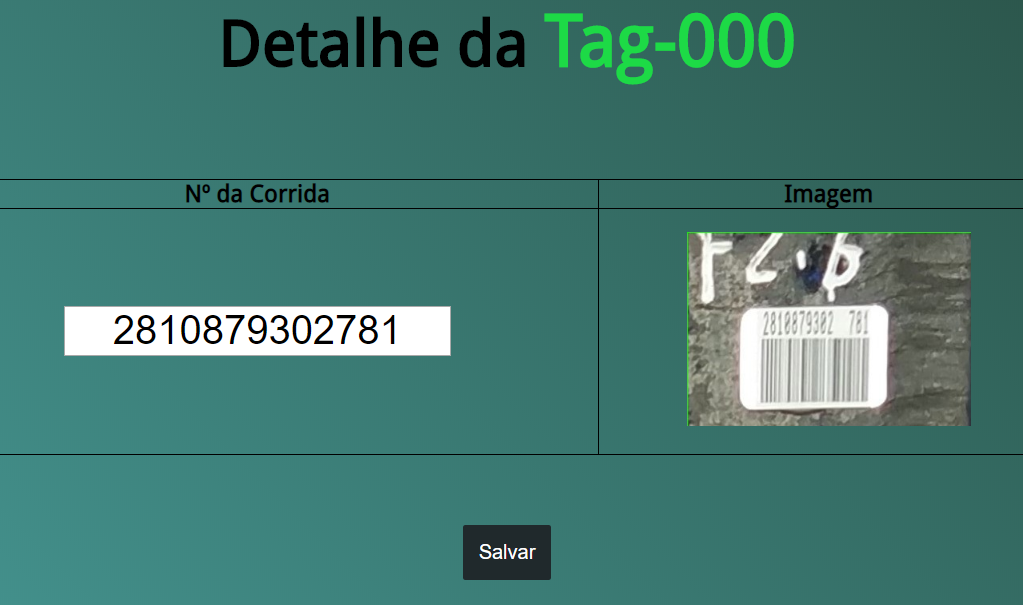
\includegraphics[width=0.8\linewidth]{figuras/WebService/Screens/detail_tag.png}
	\caption{Edição dos números da etiqueta.}
	\label{fig:detail_tag}
\end{figure}